\chapter{Convergenze di Variabili Aleatorie}

Lo studio del comportamento asintotico delle variabili aleatorie riveste un ruolo
centrale nella teoria della probabilità. Molti risultati fondamentali – come la Legge
Forte dei Grandi Numeri o il Teorema del Limite Centrale – si basano infatti sul
confronto tra successioni di variabili aleatorie e un opportuno limite.

\medskip
In questo capitolo  analizzeremo i diversi tipi di convergenza che
si possono definire nello spazio delle variabili aleatorie: la convergenza quasi
certa, la convergenza in probabilità, la convergenza in $L^{p}$ e la convergenza in probabilità. Ciascuna di esse cattura un aspetto distinto del ``tendere al limite'' e possiede proprietà e implicazioni specifiche, non sempre equivalenti tra loro.


\bigskip
\noindent Ricordiamo le definizioni di convergenza puntuale e uniforme:

\begin{definizione}[Convergenza puntuale]
    Una successione di funzioni $\{f_n\}$ converge puntualmente alla funzione $f$, per $n\to+\infty$ se:
    \[\forall \,t\in\mathbb R\qquad \lim_{n\to+\infty}f_n(t) = f(t)\]
\end{definizione}

\begin{definizione}[Convergenza uniforme]
    Una successione di funzioni $\{f_n\}$ converge uniformemente alla funzione $f$, per $n\to+\infty$ se:
    \[\forall \,t\in\mathbb R\qquad \lim_{n\to+\infty}\sup |f_n(t) - f(t)| = 0\]
\end{definizione}

\noindent Si ha ovviamente che: $\quad$ Convergenza Uniforme $\quad \Rightarrow \quad$ Convergenza Puntuale.

\bigskip
\noindent Come oramai sappiamo bene, variabili aleatorie differenti possono essere definite su spazi di probabilità differenti. È per questo motivo che andremo a suddividere la nostra analisi in due parti, analizzando prima il caso in cui abbiano stesso dominio, e poi il caso più generico.

\section{Convergenze per Variabili Reali con lo Stesso Dominio}
Avremo quindi una successione di variabili aleatorie reali $(X_n)_{n\geq1}$ definite sullo stesso spazio $(\Omega, \mathcal{A}, \mathbb{P})$.

\subsection{Convergenza Quasi Certa}

Come vedremo, la convergenza certa risulta spesso una condizione eccessivamente forte e, di conseguenza, tende a non essere soddisfatta in molti casi. Per questo motivo è necessario introdurre una nozione di convergenza ``meno stringente'', capace di catturare situazioni in cui la convergenza certa fallisce.

\begin{definizione}[Convergenza Certa]
    Diciamo che $X_n$ tende ad $X$ certamente se:
    \[\lim_{n\to+\infty}X_n(w) = X(w)\qquad \forall w\in\Omega\]
    E la indicheremo con: $\quad X_n \overset{\text{c}}{\longrightarrow}X$
\end{definizione}

La convergenza certa risulta essere la medesima della convergenza puntuale per l'analisi. Da un punto di vista modellistico può essere interpretata come segue: ogni sperimentatore osserva lo stesso limite.

\begin{definizione}[Convergenza Quasi Certa]
    Diciamo che $X_n$ tende ad $X$ quasi certamente se:
    \[\mathbb P\left(w\in\Omega: \quad \lim_{n\to +\infty}X_n (w) = X(w)\right) = 1\]
    E la indicheremo con: $\quad X_n \overset{\text{qc}}{\longrightarrow}X$
\end{definizione}

Modellisticamente parlando, si può intendere che \textit{quasi ogni} sperimentatore osserva lo stesso limite. È chiaro che per entrambe le definizioni si ha la necessità che tutte le variabili siano definite sullo stesso spazio.

\begin{esempio}
    Facciamo qualche esempio per entrare nel concreto:
    
    \bigskip
    \noindent \(\bigstar \;\) Sia $X$ una V.A. reale, e sia la successione: $\;X_n(w) = \frac{X(w)}{n} \quad \forall w\in \Omega,\;\forall n\geq1$. La successione converge? In che modo?
    \[\lim_{n \to+\infty }X_n(w) = 0\quad \forall w\in \Omega\]
    \[\Rightarrow\qquad X_n \overset{\text{c}}{\longrightarrow}0\]
    Avremo inoltre che: $\;\bigl(w\in\Omega:\;\lim_{n \to+\infty }X_n(w) = 0\bigr) = \Omega$.
        \[\Rightarrow\qquad X_n \overset{\text{qc}}{\longrightarrow}0\]

    \bigskip
    \noindent \(\bigstar \;\) Nel caso in cui si abbia convergenza monotona $X_n\uparrow X\geq0$ allora per definizione si ha che:
    \[\lim_{n\to+\infty} X_n(w) = X(w);\quad X_n\leq X_{n+1}\; \forall w\in\Omega\]
    \[\Rightarrow\qquad X_n \overset{\text{c}}{\longrightarrow}0\quad ;\quad X_n \overset{\text{qc}}{\longrightarrow}0\]

    \bigskip
    \noindent \(\bigstar \;\) Siano $\Omega = [0, 1], \;\mathcal{A} =\mathcal{B}([0, 1]), \;\mathbb P\sim \mathcal{U}([0, 1])$. Esiste quindi una densità: $\;f(t) = \mathbb{I}_{[0, 1]}(t).$ Definiamo la successione:
    \[\forall n\geq 1:\qquad X_n(w) = \mathbb{I}_{[0, \frac{1}{n}]}(w)\]
    Abbiamo due situazioni possibili:
    \begin{itemize}
        \item Se $w=0,\;$ si ha che $\;X_n(0) = 1\quad \Rightarrow\quad \lim_{n\to+\infty} X_n(0) = 1$
        \item Se $w\neq 0,\;$ si ha che $\;X_n(w) = 0 \;\forall n >\frac{1}{w}\quad \Rightarrow\quad \lim_{n\to+\infty}X_n(w) = 0$
    \end{itemize}
    Possiamo quindi dire che:
    \[\left(w\in\Omega:\;\lim_{n\to+\infty} X_n (w) = 0\right) = (0, 1]\]
    Siccome $\mathbb{P}\left((0, 1]\right) = \int_0^1 dt = 1, \;$ possiamo concludere che $\;X_n \overset{\text{qc}}{\longrightarrow}0\;$. Tuttavia non è verificata la condizione per l'uguaglianza certa per ogni $w\in\Omega\quad \Rightarrow \quad X_n \overset{\text{c}}{\nlongrightarrow}0$.

    \bigskip
    \noindent Se invece avessimo preso $\;\mathbb{P} \sim \delta_0$, allora avremmo avuto che:
    \begin{itemize}
        \item $\mathbb{P}\bigl((0, 1]\bigr) = 0$
        \item $\mathbb{P}\bigl(\{0\}\bigr) = 1$
    \end{itemize}
    \[\Rightarrow\quad \mathbb P\left(w\in\Omega:\;\lim_{n\to+\infty}X_n(w) = 1\right) = 1\quad \Rightarrow\quad X_n \overset{\text{qc}}{\longrightarrow}1\]
    
\end{esempio}

Questi esempi mostrano che \textbf{la convergenza quasi certa dipende dalla probabilità}, mentre quella certa no.

\begin{proposizione}
    Se $\qquad X_n \overset{\text{c}}{\longrightarrow}X \quad \Rightarrow\quad X_n \overset{\text{qc}}{\longrightarrow}X$.\\
    Il viceversa non è vero (si vedano gli esempi sopra).
\end{proposizione}
\bigskip
\noindent Vediamo adesso le proprietà che distinguono la convergenza quasi certa.

\begin{teorema}[Proprietà della Convergenza Quasi Certa]
\label{th:prop_conv_qc}
    Siano $(X_n)_{n\geq1}, \;(Y_n)_{n\geq1}$ successioni di variabili aleatorie, $X, \;Y$ variabili aleatorie, tutte reali e definite sullo stesso spazio di probabilità $(\Omega, \mathcal{A},\mathbb P)$. Sia inoltre $a\in\mathbb R$ e $h:\mathbb{R}\to\mathbb R$ continua.

    \medskip
    \noindent Siano le successioni tali che $X_n \overset{\text{qc}}{\longrightarrow}X$ e che $Y_n \overset{\text{qc}}{\longrightarrow}Y$, allora valgono le seguenti:
    \begin{enumerate}
        \item Il limite è unico quasi certamente. Ossia che se $\;X_n \overset{\text{qc}}{\longrightarrow}X\;$ e $\;X_n \overset{\text{qc}}{\longrightarrow}\widehat{X} \quad \Rightarrow\quad X = \widehat{X}$ q.c.
        \item $aX_n \overset{\text{qc}}{\longrightarrow}aX$
        \item $h(X_n) \overset{\text{qc}}{\longrightarrow}h(X)$
        \item $X_n + Y_n\overset{\text{qc}}{\longrightarrow}X+Y$
        \item $X_nY_n \overset{\text{qc}}{\longrightarrow}XY$
        \item $\frac{X_n}{Y_n} \mathbb{I}_{(Y_n\neq0)} \overset{\text{qc}}{\longrightarrow}\frac{X}{Y} \mathbb{I}_{(Y\neq0)}$
    \end{enumerate}

    \begin{dimostrazione}
        1. Siano $A_1, A_2$ tali che $\mathbb{P}(A_1) = \mathbb{P}(A_2) = 1$, definiti come:
        \begin{align*}
            A_1 & :=\left(w\in\Omega:\;\lim_{n\to+\infty}X_n(w) = X(w)\right)\\
            A_2 & :=\left(w\in\Omega:\;\lim_{n\to+\infty}X_n(w) = \widehat{X}(w)\right)
        \end{align*}
        Allora avremo che $\;\forall w\in A_1\cap A_2:\quad \lim_{n\to+\infty}X_n(w) = X(w) = \widehat{X}(w)$, con : $\;\mathbb{P}(A_1\cap A_2) = 1$
        \bigskip
        \noindent Le altre dimostrazioni per i punto 2. 3. 4. e 5. si svolgono nella stessa maniera.
    \end{dimostrazione}
\end{teorema}

\subsection{Convergenza in $L^p$ ed in Probabilità}

Così come abbiamo introdotto la convergenza quasi certa per gestire in modo rigoroso i casi in cui la convergenza certa fallisce, è necessario introdurre altre due nozioni di convergenza, compaiono naturalmente proprio quando la convergenza quasi certa fallisce e, oltre a ciò, si rivelano strumenti molto utili per dimostrare, in molti casi, la stessa convergenza quasi certa.

\begin{definizione}[Convergenza in $L^p$]
    Sia $1\leq p< + \infty$, diciamo che $\;X_n \overset{L^p}{\longrightarrow} X\;$ se:
    \begin{enumerate}
        \item $X_n\in L^p\quad \forall n$
        \item $X\in L^p$
        \item $\underset{n\to+\infty}{\lim}E\bigl[\left|X_n-X\right|^p\bigr] = 0\hfill \text{\small ($\forall n$ avrò una successione numerica, il cui limite deve essere zero)}$
    \end{enumerate}
\end{definizione}

Dal punto di vista modellistico, la convergenza in \(L^p\) ha un’interpretazione completamente diversa rispetto alle convergenze puntuali: ciò che controlliamo non è il comportamento di ciascun singolo osservatore, bensì il comportamento \emph{medio} dell’errore \(|X_n - X|^p\).\\
Questo significa che ``in media'' le osservazioni di \(X_n\) si avvicinano a quelle di \(X\), ma non garantisce affatto che \(X_n(w)\) converga a \(X(w)\) per ogni \(w\): il singolo osservatore può vedere oscillazioni anche molto grandi.

\[
\begin{aligned}
\text{osservatore } 1 &\longrightarrow \text{errore medio}_1\\
\vdots\\
\text{osservatore } n &\longrightarrow \text{errore medio}_n
\end{aligned}
\]

Ci aspettiamo quindi che la \emph{successione degli errori medi} converga a zero, mentre non abbiamo alcuna garanzia né informazione sul comportamento delle singole osservazioni punto per punto.


\begin{teorema}[Proprietà della Convergenza in $L^p$]
    Siano $(X_n)_{n\geq1}, \;(Y_n)_{n\geq1}$ successioni di variabili aleatorie, $X, \;Y$ variabili aleatorie, tutte reali ed appartenenti a $L^p$. Sia inoltre $a\in\mathbb R$.

    \medskip
    \noindent Siano le successioni tali che $X_n \overset{L^p}{\longrightarrow}X$ e che $Y_n \overset{L^p}{\longrightarrow}Y$, allora valgono le seguenti:
    \begin{enumerate}
        \item Il limite è unico quasi certamente. Ossia che se $\;X_n \overset{L^p}{\longrightarrow}X\;$ e $\;X_n \overset{L^p}{\longrightarrow}\widehat{X}\quad \Rightarrow\quad X = \widehat{X}$ q.c.
        \item $aX_n \overset{L^p}{\longrightarrow}aX \quad \forall a\in \mathbb R$
        \item $X_n + Y_n \overset{L^p}{\longrightarrow}X + Y$
        \item $\underset{n\to+\infty}{\lim} \E{|X_n|^p} = \E{|X|^p}\hfill \text{\small ($\E{|X_n|^p}$ è una successione numerica)}$
    \end{enumerate}
\end{teorema}

\begin{definizione}[Convergenza in Probabilità]
    Diaciamo che la successione $(X_n)_{n\geq1}$ tende ad $X$ in probabilità, per $n\to+\infty$ se:
    \[\forall \varepsilon > 0 \text{ fissato:}\qquad \lim_{n\to+\infty} \mathbb{P}\left(|X_n-X|>\varepsilon\right) = 0\]
    E la indicheremo con: $\quad X_n \overset{\mathbb{P}}{\longrightarrow}X$.
\end{definizione}

Anche in questo caso, come per la convergenza in \(L^p\), non otteniamo alcuna informazione sul comportamento del singolo osservatore.

\medskip
\noindent Da un punto di vista modellistico, possiamo immaginare che ogni osservatore calcoli l’errore \( |X_n - X| \). Ciò che analizziamo non è il valore dell’errore per un singolo osservatore, bensì la ``proporzione'' di osservatori che ottengono un errore superiore a una fissata soglia \(\varepsilon > 0\). Se questa proporzione, che è generalmente $n$--dipendente, tende a zero, allora possiamo dire che vi è convergenza in probabilità.

\begin{proposizione}
\label{prop:15.10}
Vale la seguente:
    \[X_n \overset{\mathbb{P}}{\longrightarrow}X \quad \iff \quad \lim_{n\to+\infty}\E{\frac{|X_n-X|}{1 + |X_n -X|}}  = 0\]
\end{proposizione}

Si noti che la successione di variabili aleatorie $1+|X_n-X|$ converge in $L^1$ a 0. Il denominatore rende naturalmente l'oggetto più piccolo, facilitando così la sua convergenza verso zero: potrebbero esserci situazioni in cui $\E{|X_n - X|} \nlongrightarrow
 0$, ma tutta la frazione sì.

\begin{proposizione}
\label{prop:15.11}
    Siano $(X_n)_{n\geq1}, \, X$ e $(Y_n)_{n\geq1}, \, Y$ variabili aleatorie reali, sia $a\in\mathbb{R}$ e $h:\mathbb{R}\to\mathbb{R}$ continua. 

    \medskip
    \noindent Allora valgono le stesse proprietà esposte nel Teorema \ref{th:prop_conv_qc} per la convergenza quasi certa, anche per la convergenza in probabilità.
\end{proposizione}

\bigskip
\noindent Ora che abbiamo visto che esistono vari tipi di convergenza per variabili aleatorie definite sullo stesso spazio di probabilità, vediamo quale è la relazione che intercorre tra di esse.

\begin{teorema}
\label{th:relazione_conv_A}
    Valgono le seguenti:
    \begin{enumerate}
        \item $\quad X_n \overset{\text{qc}}{\longrightarrow}X\quad \Rightarrow\quad X_n \overset{\mathbb{P}}{\longrightarrow}X$
        \item $\quad X_n \overset{L^p}{\longrightarrow}X\quad  \Rightarrow \quad X_n \overset{L^q}{\longrightarrow}X\quad \forall 1\leq q\leq p
        \quad \Rightarrow \quad X_n \overset{\mathbb{P}}{\longrightarrow}X$
    \end{enumerate}
    \begin{dimostrazione}
        1. Se $X_n \overset{\text{qc}}{\longrightarrow}X$ allora $X_n - X\overset{\text{qc}}{\longrightarrow}0$. Allora vale che:
        \[\frac{|X_n -X|}{1+ |X_n-X|} =: h(X_n-X)\quad \overset{\text{\ref{th:prop_conv_qc}}}{\Rightarrow} \quad h(X_n-X) \overset{\text{qc}}{\longrightarrow}h(0) = 0\]
        \[\Rightarrow\quad \frac{|X_n -X|}{1+ |X_n-X|} \overset{\text{qc}}{\longrightarrow}0\]
        Inoltre sappiamo che la funzione $h(X_n-X)\leq 1$ quasi certamente, allora per il teorema di convergenza dominata di Lebesgue abbiamo che:
        \[\lim_{n\to+\infty}\E{\frac{|X_n -X|}{1+ |X_n-X|}} = \E{0} = 0\]
        Per la Proposizione \ref{prop:15.10} abbiamo che: $\quad \quad X_n \overset{\mathbb{P}}{\longrightarrow}X$.

        \bigskip
        \noindent 2. La prima implicazione deriva direttamente dal fatto che gli spazi $L^p$ (nel caso di misure di probabilità) sono ``inscatolati'', ossia che $L^1 \supseteq L^2 \supseteq \cdots$

        \medskip
        \noindent Per quanto riguarda la seconda implicazione, si può notare che:
        \[\frac{|X_n -X|}{1+ |X_n-X|} \leq \frac{|X_n -X|}{1}\]
        Di conseguenza, se $\quad X_n \overset{L^1}{\longrightarrow}X\quad \Rightarrow \quad \underset{n\to+\infty}{\lim} \E{|X_n - X|} = 0$. \\
        Per il teorema del confronto:
        \[0\leq \lim_{n\to+\infty}\E{\frac{|X_n -X|}{1+ |X_n-X|}}\leq \lim_{n\to+\infty}\E{|X_n -X|} = 0\]
        E questo è vero se e solo se $\;X_n \overset{\mathbb{P}}{\longrightarrow}X$.
    \end{dimostrazione}
\end{teorema}

Questo teorema ci dice che ci sono delle convergenze naturalmente ``più forti'' di altre, e quindi esistono delle condizioni di implicazione. Si presti molta attenzione a non confondere le implicazioni, per esempio non sono vere le seguenti:
\begin{itemize}
    \item $X_n \overset{\mathbb{P}}{\longrightarrow}X \quad \not\Rightarrow \quad  X_n \overset{\text{qc}}{\longrightarrow}X$
    \item   $X_n \overset{L^p}{\longrightarrow}X \quad \not\Rightarrow \quad X_n \overset{\text{qc}}{\longrightarrow}X$
    \item   $X_n \overset{\text{qc}}{\longrightarrow}X \quad \not\Rightarrow \quad X_n \overset{L^p}{\longrightarrow}X$
\end{itemize}

\begin{teorema}
\label{th:15.13}
    Sono vere le seguenti:
    \begin{enumerate}
        \item Se $\quad X_n \overset{\mathbb{P}}{\longrightarrow}X \quad \Rightarrow\quad \exists\, (n_k)_{k\geq1}\;\text{ tale che la sottosuccessione}:\quad X_{n_k} \overset{\text{qc}}{\longrightarrow}X$
        \item Se $\;X_n \overset{\mathbb{P}}{\longrightarrow}X\;$ e $\;|X_n|\leq Y, \;\forall n\geq1\;$ con $\;Y\in L^p$. Allora:
        \begin{itemize}
            \item $X_n\in L^p\;$ e $\; X\in L^p$
            \item $X_n \overset{L^p}{\longrightarrow}X$
        \end{itemize}
    \end{enumerate}
\end{teorema}

Osservando che $|E{X_n}-\E{X}|\leq \E{|X_n-X|}$, se imponiamo $p=1$, allora otteniamo il \textit{Teorema di Lebesgue}, ma con condizioni meno stringenti (convergenza in probabilità e non quasi certa). Ossia che:

\bigskip
\noindent Se $\;X_n \overset{\mathbb{P}}{\longrightarrow}X\;$ e $\;|X_n|\leq Y, \;\forall n\geq1\;$ con $\;Y\in L^1$. Allora:
\begin{itemize}
    \item $X_n\in L^1\;$ e $\; X\in L^1$
    \item $X_n \overset{L^1}{\longrightarrow}X\quad$ che è equivalente alla condizione di Lebesgue: $\quad \underset{n\to+\infty}{\lim}\E{X_n} = \E{X}$
\end{itemize}

\section{Teoremi Limite: Legge Debole e Forte dei Grandi Numeri}

I teoremi limite rappresentano alcuni dei risultati più profondi e potenti della Teoria della Probabilità. Essi descrivono il comportamento di successioni di variabili aleatorie quando il numero di osservazioni cresce, e forniscono le basi matematiche per molte intuizioni statistiche fondamentali.

\medskip
Partendo da ipotesi spesso molto deboli, questi risultati gettano le fondamenta concettuali della statistica moderna: mostrano infatti in che modo l’informazione campionaria si “stabilizza” e perché certe approssimazioni diventano affidabili quando il numero di osservazioni cresce. Tutte le dimostrazioni poggiano sulla teoria sviluppata finora — in particolare sulla convergenza di variabili aleatorie — ma, giunti a questo punto della trattazione, appariranno sorprendentemente concise e naturali.\\
\\
Data $(X_n)_{n\geq 1}$ una successione di variabili aleatorie definite sullo
stesso spazio di probabilità, e consideriamo la somma parziale o la media campionaria
\[
    S_n = \sum_{k=1}^n X_k \qquad ;\qquad \frac{1}{n} S_n
\]

i risultati che descrivono la convergenza di tali quantità, in uno dei sensi
di convergenza introdotti nei capitoli precedenti, prendono il nome di
\emph{Legge dei Grandi Numeri}.

\begin{teorema}[Legge Debole dei Grandi Numeri]
    Sia $(X_n)_{n\geq 1}$ una successione di variabili aleatorie reali definite sullo stesso spazio di probabilità $(\Omega, \mathcal{A}, \mathbb{P})$ tali che $X_n\in L^2(\Omega, \mathcal{A}, \mathbb{P})\quad \forall n\geq1\;$ e che valgano:
    \begin{enumerate}
        \item $\E{X_n} = \mu \quad \forall n$
        \item $Var(X_n) = \sigma_n^2 \leq \sigma ^2 \quad $ per un qualche $\;0<\sigma^2<+\infty$
        \item Vale il limite:\[\lim_{n\to+\infty} n^{-2} \sum_{1\leq k<h\leq n} \bigl|\rho (X_h, X_k)\bigr| = 0\]
    \end{enumerate}
    Allora si ha che la media campionaria $\;\overline{X}_n = \frac{(X_1+\cdots +X_n)}{n} \;\forall n\geq 1$ è tale che:
    \[\boxed{\overline{X}_n \overset{L^2}{\longrightarrow}\mu\qquad \text{e} \qquad \overline{X}_n \overset{\mathbb{P}}{\longrightarrow}\mu}\]
    \begin{dimostrazione}
        Ci basta studiare i comportamenti asintotici di media e varianza di $\overline{X}_n$.
        \[\E{\overline{X}_n} = \frac{\E{X_1 +\cdots +X_n}}{n} = \frac{n\mu}{n} = \mu\]
        Per quanto riguarda la varianza, ricordando che $\rho (X_h, X_k) \sigma_k\sigma_h = Cov(X_h, X_k)$, si ottiene:
        \begin{align*}
            Var\left(\overline{X}_n\right) & = \frac{Var(X_1+\cdots+X_n)}{n^2} = \frac{1}{n^2}\left[\sum_{k=1}^n Var(X_k) + 2\sum_{1\leq k<h\leq n}Cov(X_h, X_k)\right] \\
            & = \frac{1}{n^2}\left[\sum_{k=1}^n\sigma_k^2 + 2 \sum_{1\leq k<h\leq n} \rho (X_h, X_k) \sigma_k\sigma_h\right] \\ 
            & \leq \frac{1}{n^2} \left[ n \sigma^2 + 2\sigma^2\sum_{1\leq k<h\leq n} \rho (X_h, X_k)\right] && \!\!\!\!\!\!\!\!\!\!\!\!\left(\textit{Siccome:}\;\sigma_k^2\leq \sigma^2\right)\\
            & = \frac{\sigma^2}{n} + 2\sigma^2 \;\underbrace{n^{-2} \left[\sum_{1\leq k<h\leq n} \rho (X_h, X_k)\right]}_{\longrightarrow \,0 \;\text{ per ipotesi}} \underset{n\to+\infty}{\longrightarrow }0
        \end{align*}
        $\Rightarrow \quad Var\left(\overline{X}_n\right) \longrightarrow 0$

        \medskip
        \noindent Avremo allora che, siccome $\E{\overline{X}_n} = \mu$:
        \begin{align*}
            \left\|\overline{X}_n - \mu\right\|_{L^2}^2 & = \E{\left(\overline{X}_n - \mu\right)^2} = \E{\overline{X}_n^2} + \mu^2 - 2\mu \E{\overline{X}_n}\\
            & = \E{\overline{X}_n^2} - E^2\left[\overline{X}_n\right]\\
            & = Var(\overline{X}_n) \longrightarrow 0
        \end{align*}
        Abbiamo appena dimostrato che: $\quad \overline{X}_n \overset{L^2}{\longrightarrow}\mu$, e di conseguenza, avremo che $\quad \overline{X}_n \overset{\mathbb P}{\longrightarrow}\mu$ 
    \end{dimostrazione}
\end{teorema}

Si osservi che non si chiede che le $(X_n)_{n\geq1}$ siano una famiglia di variabili indipendenti ed identicamente distribuite (i.i.d.), difatti nel punto 2. le $\sigma_n^2$ possono essere diverse.

\medskip
\noindent Si può inoltre notare che il limite nel punto 3. non chiede altro che la successione dipendente da $n$ in sommatoria, sia un $o(n^2)$

\bigskip
\noindent Da questo teorema possiamo dedurre due importanti corollari.

\begin{corollario}
\label{cor:15.15}
    Sia $(X_n)_{n\geq1}$ una successione di variabili aleatorie identicamente distribuite\footnote{Ossia che $P^{X_n}\sim P^{X}\quad \forall n$} tali che $\;Cov(X_h, X_k) = 0\quad \forall h\neq k, \; X_n\in L^2, \;\E{X_n} = \mu$. 

    \medskip Allora avremo che:
    \[\overline{X}_n \overset{L^2}{\longrightarrow}\mu \quad \text{e}\quad \overline{X}_n \overset{L^1}{\longrightarrow}\mu\quad \text{e}\quad \overline{X}_n \overset{\mathbb{P}}{\longrightarrow}\mu \]
    \begin{dimostrazione}
        Il fatto che siano i.d. implica che $Var(X_n) = \sigma^2 < +\infty.$ Inoltre essendo la $Cov(X_h, X_k) = 0, $ la sommatoria (nella condizione 3.) risulta essere zero, valendo così la legge debole dei grandi numeri.
    \end{dimostrazione}
\end{corollario}

\begin{corollario}
\label{cor:15.16}
    Sia $(X_n)_{n\geq1}$ una successione di variabili aleatorie indipendenti identicamente distribuite, con $X_n\in L^2\quad \forall n, $ tale che $\E{X_n} = \mu$ e $Var(X_n) = \sigma^2 \in [0, +\infty)$.

    \medskip Allora avremo che:
    \[\overline{X}_n \overset{L^2}{\longrightarrow}\mu \quad \text{e}\quad \overline{X}_n \overset{L^1}{\longrightarrow}\mu\quad \text{e}\quad \overline{X}_n \overset{\mathbb{P}}{\longrightarrow}\mu \]
    \begin{dimostrazione}
        Essendo indipendenti, la covarianza sarà zero per ogni coppia, valendo così il corollario \ref{cor:15.15}.
    \end{dimostrazione}
\end{corollario}

\bigskip \noindent Prima di introdurre la legge forte dei grandi numeri, enunciamo un lemma fondamentale che ci aiuterà nella dimostrazione.
\begin{lemma}
\label{lemma:15.17}
    Sia $(Y_n)_{n\geq1}$ una successione di variabili aleatorie reali tali che $Y_n\geq 0\;$ q.c.$\:\forall n$. 

    \medskip \noindent Allora:

    \[\E{\sum_{n = 1}^{+\infty} Y_n} = \sum_{n = 1}^{+\infty}\E{Y_n}\]

    \begin{dimostrazione}
        Se $Y_n\geq 0 \quad \Rightarrow\quad \sum_{n = 1}^k Y_n \;\uparrow\;\sum_{n = 1}^{+\infty} Y_n\;$ per $k\to+\infty$.

        \medskip \noindent Posso usare il Teorema di Beppo Levi:
        \begin{align*}
            \E{\lim_{k\to+\infty}\sum_{n = 1}^{k}Y_n} & = \lim_{k\to+\infty} \E{\sum_{n = 1}^{k} Y_n} \\
            & = \lim_{k\to+\infty} \sum_{n = 1}^{k} \E{Y_n} &&\textit{\small(Per linearità della media)}\\
            & = \sum_{n = 1}^{+\infty} \E{Y_n}
        \end{align*}
    \end{dimostrazione}
\end{lemma}

Questo assicura la linearità dell'integrale (o del valore atteso) anche per somme infinite, qualora sia rispettata l'ipotesi. Infatti, se avevamo già visto che il valore atteso è una mappa lineare per somme finite, questo non è sempre vero per somme infinite, ma abbiamo la necessità di poter scambiare il segno di limite con quello di integrale; questo è garantito dal teorema di Beppo Levi.

\begin{teorema}[Legge Forte dei Grandi Numeri (LFGN)]
    Sia $(X_n)_{n\geq 1}$ na successione di variabili aleatorie reali definite sullo stesso spazio di probabilità $(\Omega, \mathcal{A}, \mathbb{P})$ tale che:
    \begin{enumerate}
        \item $X_n$ siano i.i.d.
        \item $\E{X_n} = \mu \;$ e $\; Var(X_n) = \sigma^2\in [0, +\infty)$
    \end{enumerate}
    Allora si ha che:
    \[\overline{X}_n \overset{\text{qc}}{\longrightarrow}\mu \qquad \text{(e anche in $L^2$)}\] 
\end{teorema}
\begin{dimostrazione}
        Senza perdere di generalità poniamo $\mu = 0$ (se si volesse $\mu\neq 0$ basterebbe eseguire la stessa dimostrazione utilizzando $Y_n = X_n - \mu$).

        \medskip \noindent $(*)$ Per il corollario \ref{cor:15.16} si ha che $\overline{X}_n \overset{L^2}{\longrightarrow}0$.
        
        \medskip \noindent $(* *)$ Siccome converge in $L^2$, allora convergerà anche in probabilità, e quindi esiste una sottosuccessione che converge quasi certamente. Si vuole quindi trovare la sottosuccessione che converge quasi certamente a $\mu = 0$. Definisco allora:
        \[Y_n : = \overline{X}_{n^2} = \frac{X_1 + \cdots + X_{n^2}}{n^2} \quad \Rightarrow\quad (Y_1, Y_2, Y_3, \cdots ) = (\overline{X}_1, \overline{X}_4, \overline{X}_9, \cdots)\]
        Si osserva che:
        \[\text{Se: }\; \sum_{n=1}^{+\infty} Y_n^2(w) < + \infty \text{ q.c.}\quad \Rightarrow\quad \lim_{n\to+\infty} Y^2_n(w) = 0 = \lim_{n\to+\infty} Y_n(w)\]
        
        siccome è il termine generale di una serie convergente.
        
        \medskip \noindent Allora ci basta dimostrare che la serie non diverga:
        \begin{align*}
            \E{\sum_{n=1}^{+\infty} Y_n^2} & \overset{\text{\ref{lemma:15.17}}}{=} \sum_{n=1}^{+\infty} \E{Y_n^2} = \sum_{n=1}^{+\infty} \E{\overline{X}_{n^2}^2} \\
            & \overset{\mu = 0}{=} \sum_{n=1}^{+\infty}Var(\overline{X}_{n^2})  = \sum_{n=1}^{+\infty}\left(\frac{Var(X_1+\cdots+X_{n^2})}{n^4}\right) \\
            & = \sum_{n=1}^{+\infty}\frac{1}{n^4}n^2\sigma^2 \\
            & = \sum_{n=1}^{+\infty}\frac{\sigma^2}{n^2} < +\infty \\
            & \Longrightarrow \sum_{n=1}^{+\infty} Y_n^2 < +\infty \quad \text{q.c.}
        \end{align*}
        \[\Rightarrow \quad \mathbb P\left(w\in \Omega:\; \sum_{n=1}^{+\infty}Y_n^2 (w) <+\infty \right) = 1 \quad \Rightarrow \quad \lim_{n\to+\infty} Y^2_n(w) = 0 = \lim_{n\to+\infty} Y_n(w)\;\text{q.c.}\]

        \bigskip
        \noindent $(*\!*\!*)$ Abbiamo quindi trovata la sottosuccessione che converge quasi certamente alla media, tuttavia noi vogliamo dimostrare che tutta la successione converga quasi certamente. 
        
        \medskip \noindent Poniamo $\forall n\geq1:\quad p(n) = \left\lfloor \sqrt{n}\right\rfloor$. Allora avremo che:
        \begin{equation}
        \label{eq:dim_leggeforte}
            \left(\sqrt{n}-1\right)^2\leq p(n)^2\leq n \quad \Rightarrow \quad \frac{\left(\sqrt{n}-1\right)^2}{n}\leq \frac{p(n)^2}{n}\leq \frac{n}{n} = 1
        \end{equation}

        Questo prova che $\overline{X}_{p(n)^2}$ è una sottosuccessione di $\overline{X}_{n^2}:\quad \left(\overline{X}_{p(n)^2}:\;n\geq 1\right)\subseteq \left(\overline{X}_{n^2}:\;n\geq 1\right)$.\\
        Per esempio abbiamo che: 
        \[\overline{X}_{p(1)^2} = \overline{X}_{1};\quad \overline{X}_{p(2)^2} = \overline{X}_{1};\quad \overline{X}_{p(3)^2} = \overline{X}_{1};\quad  \overline{X}_{p(4)^2} = \overline{X}_{4};\quad \cdots\]

        Allora, per il passo $(**)$, si ha che $\quad \overline{X}_{p(n)^2}\overset{\text{qc}}{\longrightarrow} 0.$

        \medskip
        Possiamo riscrivere la media campionaria come: 
        \[\overline{X}_n = \underbrace{\overline{X}_n - \frac{p(n)^2}{n}\overline{X}_{p(n)^2}}_{:= V_n} + \underbrace{\frac{p(n)^2}{n}}_{\leq 1} \;\underbrace{\overline{X}_{p(n)^2}}_{\to\;0}\]

        Il secondo ``pezzo'' della media campionaria tende a zero quasi certamente, perché $\overline{X}_{p(n)^2}\overset{\text{qc}}{\longrightarrow}0$ e $\frac{p(n)^2}{n}\leq 1$. Se riusciamo a dimostrare che anche $V_n$ tende q.c. a 0, allora abbiamo dimostrato la tesi.

        \medskip
        Come fatto nel passo $(**)$, se riusciamo a dimostrare che $\sum_{n=1}^{+\infty} \E{V_n^2}<+\infty$, allora abbiamo garantito che $V_n\overset{\text{q.c}}{\longrightarrow} 0.$ Riscriviamo in maniera più comoda $V_n$:
        \[V_n = \overline{X}_n - \frac{p(n)^2}{n}\overline{X}_{p(n)^2} = \frac{1}{n}\sum_{k=1}^n X_k - \frac{p(n)^2}{n}\cdot \frac{1}{p(n)^2}\cdot \sum_{k=1}^{p(n)^2}X_k = \frac{1}{n}\sum_{k = p(n)^2 + 1}^n X_k\]

        Calcoliamo a questo punto $\E{V_n^2}:$
        \begin{align*}
            \E{V_n^2} & = \E{\left(\frac{1}{n} \sum_{k = p(n)^2 + 1}^n X_k\right)^2} = \frac{1}{n^2} \sum_{k = p(n)^2 + 1}^n \E{X_k^2} \\
            & = \frac{1}{n^2} \sigma^2 \left(n-p(n)^2\right) \\
            & \overset{\text{\eqref{eq:dim_leggeforte}}}{\leq} \frac{\sigma^2}{n^2}\left(n - (\sqrt{n}-1)^2\right) = \frac{\sigma^2}{n^2}(n-n+2\sqrt{n} - 1)\\
            & \leq 2\sigma^2 \frac{\sqrt{n}}{n^2} = n^{-3/2}
        \end{align*}
        \begin{align*}
            & \Longrightarrow \quad \sum_{n=1}^{+\infty} \E{V_n^2}\leq 2\sigma\sum_{n=1}^{+\infty}n^{-3/2} <+\infty \quad \Rightarrow\quad V_n^2\overset{\text{qc}}{\longrightarrow} 0\\
            & \Longrightarrow \quad \lim_{n\to+\infty} V_n = \lim_{n\to+\infty}\overline{X}_n - \frac{p(n)^2}{n}\overline{X}_{p(n)^2} = 0 \quad \text{q.c.}\\
            & \Longrightarrow \quad \overline{X}_n = V_n + \frac{p(n)^2}{n}\overline{X}_{p(n)^2} \overset{\text{qc}}{\longrightarrow} 0
        \end{align*}
    \end{dimostrazione}
Questo teorema è definito ``forte'' proprio perché ci assicura una convergenza quasi certa, che è più forte della convergenza in $L^p$ o in probabilità.

\begin{figure}[H]
    \centering
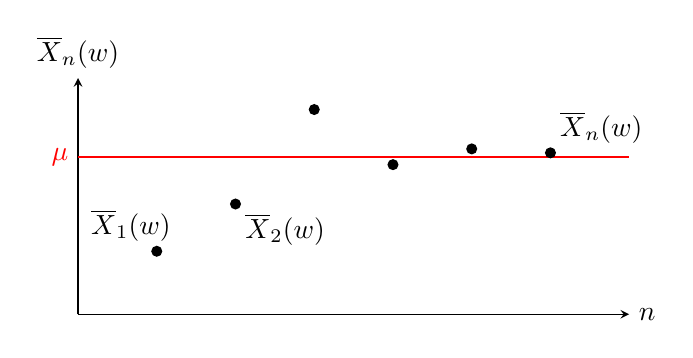
\begin{tikzpicture}[>=stealth, scale=1]

%------------------------------------------------
% PANNELLO ALTO: traiettoria delle medie campionarie
%------------------------------------------------
% Assi
\draw[->] (0,0) -- (7,0) node[right] {$n$};
\draw[->] (0,0) -- (0,3) node[above] {$\overline{X}_n(w)$};

% Retta della media vera mu
\draw[red, thick] (0,2) -- (7,2);
\node[left, red] at (0,2) {$\mu$};

% Alcuni punti della traiettoria delle medie
\fill (1,0.8) circle (2pt);
\fill (2,1.4) circle (2pt);
\fill (3,2.6) circle (2pt);
\fill (4,1.9) circle (2pt);
\fill (5,2.1) circle (2pt);

% Ultimo punto "vicino" a mu con etichetta generica
\fill (6,2.05) circle (2pt);
\node[above right] at (6,2.05) {$\overline{X}_n(w)$};

% Etichette per i primi due punti (facoltative)
\node[above left]  at (1.3,0.8) {$\overline{X}_1(w)$};
\node[below right] at (2,1.4) {$\overline{X}_2(w)$};
    \end{tikzpicture}
    \caption{Rappresentazione grafica della LFGN}
\end{figure}

\subsection{Applicazione: Funzione di Ripartizione Empirica}
In quasi tutti i contesti reali, l’unica informazione realmente disponibile su una variabile aleatoria proviene dai campioni osservati. Un problema naturale è dunque capire in che modo le frequenze osservate si comportino rispetto alle probabilità teoriche: \textit{è possibile descrivere la distribuzione di una variabile aleatoria soltanto a partire dai dati?}

\medskip
La funzione di ripartizione empirica nasce esattamente per rispondere a questa domanda: si tratta quindi di un oggetto interamente costruito sui dati, privo di qualsiasi conoscenza a priori sulla distribuzione teorica.


\bigskip
\noindent Supponiamo quindi di avere un campione statistico $(X_n)_{n\geq1}$ i.i.d. e definiamo la funzione di ripartizione per ogni $n$ come $F_{X_n} = F_X$. Possiamo costruire la successione di funzioni $F_n$ tale che:

\[\forall t\in\mathbb R\qquad F_n(t) = \frac{1}{n}\sum_{k=1}^n \mathbb{I}_{(-\infty, t]}(X_k)\qquad \text{``}=\text{''}\; \frac{\text{\# Osservazioni in } (-\infty, t]}{n}\]

Questa è proprio detta \textit{Funzione di Ripartizione Empirica}, che rappresenta $\;\forall w\;$la frequenza relativa della classe $(-\infty, t]$.  Si presti attenzione che $F_n$ è una funzione aleatoria, difatti dipende anche da $w$ e non solo da $t$; per essere formalmente corretti, bisognerebbe definirla come:
\[\boxed{F_n(t, w) = \frac{1}{n}\sum_{k=1}^n \mathbb{I}_{(-\infty, t]}\bigl(X_k(w)\bigr)}\]
Poiché il valore della funzione dipende dall’esito elementare $w$: la variabile
$X_k = X_k(w)$ può essere inclusa oppure no nell’indicatrice
$\mathbb{I}_{(-\infty, t]}(X_k)$ e quindi contribuire o meno al conteggio.

\medskip
Per comprenderne la struttura, consideriamo un singolo osservatore (cioè un
singolo $w$) per il quale le $n$ osservazioni risultino tutte distinte.
Ordinando gli $X_k$ dal più piccolo al più grande sull’asse delle ascisse, la
funzione empirica presenta esattamente $n$ discontinuità, una in
corrispondenza di ciascun valore osservato, e ciascun salto ha ampiezza $1/n$. Se alcune osservazioni coincidono, ad esempio $m$ valori identici, il numero di
salti si riduce a $n-m$, mentre il salto in corrispondenza del valore ripetuto
diventa più grande, pari a $m/n$.

\bigskip
\noindent 
In ogni caso, il grafico di $F_n$ dipende sia dall’esito realizzato sia dal numero
$n$ di osservazioni disponibili: la famiglia $(F_n)_{n\ge 1}$ costituisce quindi
una successione di \emph{funzioni aleatorie}, una per ciascun esperimento
effettuato.

\begin{esempio}
    Si consideri $n=4$. Supponiamo che si osservino $X_1(w), X_2(w), X_3(w), X_4(w)$. Allora possiamo costruire la funzione di ripartizione empirica come segue:

    \[
    F_4(t)(w)=
    \begin{cases}
    0, & t < X_{4}(w),\\[4pt]
    \frac14, & X_{4}(w) \le t < X_{3}(w),\\[4pt]
    \frac12, & X_{2}(w) \le t < X_{1}(w),\\[4pt]
    \frac34, & X_{1}(w) \le t < X_{3}(w),\\[4pt]
    1, & t \ge X_{3}(w).
    \end{cases}
    \]
    Il cui grafico risulta essere:
    \begin{figure}[H]
        \centering
        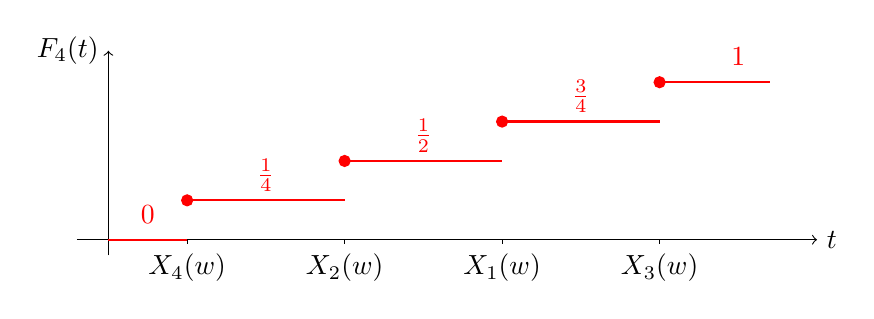
\begin{tikzpicture}[xscale=2, yscale=2]
    % Assi
    \draw[->] (-0.2,0) -- (4.5,0) node[right] {$t$};
    \draw[->] (0,-0.1) -- (0,1.2) node[left] {$F_4(t)$};

    % Punti ordinati X1 < X2 < X3 < X4
    \foreach \x/\lab in {0.5/{X_{4}(w)}, 1.5/{X_{2}(w)}, 2.5/{X_{1}(w)}, 3.5/{X_{3}(w)}} {
        \draw (\x,0) -- (\x,-0.03);
        \node[below] at (\x,-0.03) {$\lab$};
    }

    % Segmenti orizzontali
    \draw[red, thick] (0,0) -- (0.5,0);
    \draw[red, thick] (0.5,0.25) -- (1.5,0.25);
    \draw[red, thick] (1.5,0.5) -- (2.5,0.5);
    \draw[red, thick] (2.5,0.75) -- (3.5,0.75);
    \draw[red, thick] (3.5,1) -- (4.2,1);

    % Salti (cerchi aperti/chiusi)
    \foreach \x/\y in {0.5/0.25, 1.5/0.5, 2.5/0.75, 3.5/1} {
        \filldraw[red] (\x,\y) circle (1pt);
    }

    % Etichette dei livelli
    \node[red] at (0.25,0.16) {$0$};
    \node[red] at (1,0.25+0.16) {$\frac14$};
    \node[red] at (2,0.5+0.16) {$\frac12$};
    \node[red] at (3,0.75+0.16) {$\frac34$};
    \node[red] at (4,1+0.16) {$1$};
\end{tikzpicture}
    \end{figure}
\end{esempio}

Convinti del fatto, per ogni $t\in\mathbb R$ fissato, $F_n$ è una successione di variabili aleatorie, possiamo riconoscergli le seguenti proprietà.
\begin{enumerate}
    \item Posso definire $Y_k := \mathbb{I}_{(-\infty, t]}(X_k)$, con $(X_n)_{n\geq1}$ i.i.d., allora la fdr empirica diventa:
    \[F_n(t) = \frac{Y_1 + \cdots + Y_n}{n}\]
    $\Rightarrow\quad (Y_n)_{n\geq1}\;$ è i.i.d. tale che $\quad Y_k \sim Be\bigl(F_X(t)\bigr)$
    \item $\E{F_n(t)} = \E{Y_1} = F_X(t)$
    \item $\begin{aligned}Var\bigl(F_n(t)\bigr) = \frac{F_X(t)\bigl(1-F_X(t)\bigr)}{n}\end{aligned}$
    \item Per LFGN: $\quad \forall t\quad F_n(t, w) = \overline{Y}_n \overset{\text{qc}}{\longrightarrow}F_X(t)$
\end{enumerate}

\begin{teorema}[Glivencko--Cantelli]
    Sia $(X_n)_{n\ge1}$ una successione di variabili aleatorie reali i.i.d. con
    funzione di ripartizione $F_X(t)$ con $t\in\mathbb{R}$, allora:
    \[\sup_{t\in\mathbb R}\bigl|F_n(t, w) - F_X(t)\bigr| \overunderset{\text{qc}}{n}{\longrightarrow} 0\]
\end{teorema}

Possiamo ora cogliere la profonda differenza tra la LFGN (punto 4 dell’elenco
precedente) e il Teorema di Glivenko--Cantelli. La LFGN garantisce, per ogni
$t$ fissato, una convergenza \emph{punto per punto} con probabilità $1$; in altre
parole, per ogni valore di soglia considerato singolarmente si ha $F_n(t)\to F_X(t)$
quasi certamente.

\medskip
\noindent 
Il Teorema di Glivenko--Cantelli è invece molto più forte: non si limita a fissare
un singolo valore di $t$, ma considera \emph{tutti} i valori reali simultaneamente e
afferma che la convergenza è \emph{uniforme}. In questo senso, l’intero grafico della funzione di ripartizione empirica finisce per “aderire” uniformemente a quello della funzione di ripartizione teorica.

\medskip
$\Rightarrow\quad $ \textbf{Passiamo da una convergenza puntuale (LFGN) ad una uniforme (GC)}

\bigskip
\noindent È proprio grazie al Teorema di Glivenko--Cantelli che possiamo giustificare teoricamente il perché gli ``istogrammi approssimano la distribuzione reale'' all'aumentare di $n$. Infatti, poiché la funzione di ripartizione empirica $F_n$ converge uniformemente a $F_X$, le frequenze empiriche sugli intervalli --- da cui l’istogramma è
costruito --- convergono alle probabilità teoriche degli stessi intervalli, fornendo
così una stima coerente della densità (quando esiste).

\section{Convergenza in Legge}
Fino ad ora abbiamo studiato il caso in cui tutte le variabili aleatorie considerate esistessero sullo stesso dominio. In questo capitolo affronteremo invece il caso in cui siano definite su domini differenti, ossia che si abbiano
\begin{align*}
     X_n &: (\Omega_n, \mathcal{A}_n, \mathbb{P}_n)\to (\mathbb R, \mathcal{B})\\
     X &: (\Omega, \mathcal{A}, \mathbb{P})\to (\mathbb R, \mathcal{B})
\end{align*}

È immediato che le convergenze introdotte fino ad adesso non abbiano più alcun senso matematico, in quanto l'espressione ``$X_n(w) - X(w)$'' perde di significato, siccome gli $w$ sono moralmente diversi.

\bigskip
\noindent Dovremo quindi cambiare radicalmente il modo di pensare, ed andare a lavorare sui codomini: la nozione di convergenza, nel caso di domini differenti, coinvolgerà indubbiamente le leggi $P^{X_k}$ e $P^X$ (che ricordiamo essere misure di probabilità sui codomini).

\begin{definizione}[Convergenza Debole]
    Siano $(\mathbb Q_n)_{n\geq1}$ e $\mathbb Q$ misure di probabilità su $\mathcal{B}$. Diciamo che $\mathbb{Q}_n$ converge debolmente a $\mathbb{Q}$ se: 
    \[\forall h\in C_b^0(\mathbb R)\quad \text{vale che}\qquad \int_\mathbb{R}h(x)\;d\mathbb{Q}_n \underset{n\to+\infty }{\longrightarrow} \int_\mathbb{R}h(x)\;d\mathbb{Q}\]

    E la indicheremo con: $\quad \mathbb Q_n\overset{D}{\longrightarrow}\mathbb Q$.

    \bigskip

    \footnotetext{$C_b^0(\mathbb{R}) = \{f:\mathbb{R}\to \mathbb R \mid \text{ continua e limitata}\}$}    
\end{definizione}

In un certo senso la convergenza debole ``cerca di imitare'' la convergenza punto per punto. Per capire meglio cosa si intende, si consideri $(x_n)_n,\;x_n\in\mathbb R$ tale che $x_n\longrightarrow x.$ Allora, se definiamo $\mathbb Q_n := \delta_{x_n}$ e $\mathbb Q := \delta_x$ e ipotizziamo che $\mathbb Q_n\overset{D}{\longrightarrow}\mathbb Q$:

\[\int_\mathbb{R}h(y)\;d\mathbb{Q}_n(y) = h(x_n) \underset{n\to+\infty}{\longrightarrow} h(x) = \int_\mathbb{R}h(y)\;d\mathbb{Q}(y)\]

Quindi la convergenza debole è una generalizzazione della convergenza dei punti reali: quando le misure sono Dirac, convergere debolmente equivale semplicemente a far convergere i punti dove le Dirac sono concentrate.

\begin{definizione}[Convergenza in Legge]
    Siano $X_n, X$ variabili aleatorie con rispettivamente $P^{X_n}, P^X.$ Diciamo che $X_n\overset{\mathcal{L}}{\longrightarrow} X$ in Legge se:

    \[P^{X_n} \overset{D}{\longrightarrow} P^X\]

    Ossia che: $\quad \begin{aligned}\forall h\in C_b^0(\mathbb R)\qquad \int_\mathbb{R}h(x)\;dP^{X_n} \underset{n\to+\infty }{\longrightarrow} \int_\mathbb{R}h(x)\;dP^X\end{aligned}$
\end{definizione}

\begin{proposizione}
\label{prop:15.22}
    \[\boxed{X_n\overset{\mathcal{L}}{\longrightarrow} X\quad \iff \quad E_n\left[h(X_n)\right] \longrightarrow \E{h(X)}\quad \forall h\in C^0_b(\mathbb{R})}\]

    \begin{dimostrazione}
        L'implicazione $(\Rightarrow)$ è banalmente verificata dalla definizione di convergenza in legge.

        \medskip
        \noindent Per quanto riguarda $(\Leftarrow)$ si ha che:
        \begin{align*}
        E_n\left[h(X_n)\right] & = \int_{\Omega_n} h\left(X_n\right)\;d\mathbb{P}_n = \int_\mathbb{R} h\;dP^{X_n} \\
        & \!\!\!\!\!\!\!\!\!\!\!\!\!\!\!\Big\downarrow \; \textit{\small$\forall h\in C^0_b(\mathbb{R})$}\\
        \E{h(X)} & = \int_{\Omega} h\left(X\right)\;d\mathbb{P} = \int_\mathbb{R} h\;dP^{X}
        \end{align*}
        \[\Rightarrow\qquad \int_\mathbb{R} h\;dP^{X_n} \longrightarrow \int_\mathbb{R} h\;dP^{X}\qquad \forall h\in C^0_b(\mathbb{R})\]
        Ossia che: $P^{X_n}\overset{D}{\longrightarrow} P^X \quad \Rightarrow\quad X_n\overset{\mathcal{L}}{\longrightarrow} X$
    \end{dimostrazione}
\end{proposizione}

\bigskip
\noindent \faWarning $\;$ Con questa proposizione non stiamo assolutamente dicendo che $\E{X_n}\longrightarrow \E{X}$. Quindi:
\[X_n\overset{\mathcal{L}}{\longrightarrow} X \quad \nLongrightarrow\quad \E{X_n}\longrightarrow \E{X}\]
\begin{esempio}
    Sia $X_n$ la successione di variabili aleatorie tale che:
    \[X_n = \begin{cases}
        n, \qquad \text{con probabilità } \;\frac{1}{n}\\
        0, \qquad \text{con probabilità } \;1-\frac{1}{n}
    \end{cases}\]

    Il calcolo dell'attesa è molto semplice: \(\quad \E{X_n} = n\cdot \frac1n + 0\cdot \left(1-\frac1n\right) = 1\).\\
    Se consideriamo $h\in C^0_b:\qquad \E{h(X_n)} = h(n)\frac1n + h(0)\left(1-\frac1n\right)$.

    \medskip
    La variabile limite, se esiste, deve essere $X\equiv0$, perché è facile vedere che $X_n\overset{\mathbb{P}}{\longrightarrow} 0$. 
    \[\Rightarrow\quad \Bigl|\E{h(X_n)} - \E{h(X)}\Bigr| = \left|\bigl[h(n) - h(0)\bigr]\frac1n\right|\leq \frac{2M}n \longrightarrow 0\]
    Dove la disuguaglianza finale è stata possibile ricordandoci che $h$ è limitata, ossia che $|h(x)|\leq M\;\forall x\in\mathbb{R}$.
    \[\Rightarrow\quad X_n\overset{\mathcal{L}}{\longrightarrow} 0\quad \text{ma} \quad \E{X_n} \longrightarrow 1\]
\end{esempio}

\bigskip
\noindent È importante sottolineare che \textbf{il limite in legge è unico esclusivamente in legge}, ossia:
\[X_n\overset{\mathcal{L}}{\longrightarrow} X \quad \text{e} \quad X_n\overset{\mathcal{L}}{\longrightarrow} \widehat{X} \quad \Rightarrow\quad X \sim \widehat{X}\quad \text{(Ossia che hanno stessa legge)}\]
Ma non è assolutamente vero che $X(w) = \widehat{X}(w)$ q.c.

\bigskip
\begin{esempio}
    Facciamo un controesempio per convincerci di questo fatto. Consideriamo
    \[X\sim Be(1/2)\qquad Y = 1 -X \sim Be(1/2)\]
    Avremo quindi che $\mathbb{P}\bigl(w:\;X(w) = Y(w)\bigr) = 0$, in quanto se $X=1$, allora $Y=0$. Se introduciamo la successione $X_n = X \;\forall n$ allora avremo che $X_n \overset{\mathcal{L}}{\longrightarrow}X$ ma anche $X_n \overset{\mathcal{L}}{\longrightarrow}Y$.

    \medskip
    Abbiamo appena dimostrato che $P^X = P^Y$, ma $X\neq Y\;\forall w$.
\end{esempio}

\begin{teorema}
\label{th:15.23}
    Siano $(X_n), X$ variabili aleatorie reali, con rispettivamente $F_{X_n}, F_X$ le loro funzioni di ripartizione. 
    
    \medskip Allora:
    \[X_n \overset{\mathcal{L}}{\longrightarrow}X \quad \iff \quad F_{X_n}(t)\longrightarrow F_X(t) \quad \forall \text{ Punto di continuità $t$ di } F_X(t)\]
\end{teorema}

\noindent Analizziamo separatamente il caso continuo da quello discreto:
\begin{itemize}
    \item Se $X$ è assolutamente continua, allora avremo che $F_X$ è continua, quindi:
    \[X_n \overset{\mathcal{L}}{\longrightarrow}X \quad \iff \quad F_{X_n}(t)\longrightarrow F_X(t) \quad \text{puntualmente } \forall t\in\mathbb{R}\]
    \noindent Allora posso dire che $\;P^{X_n}(I) \longrightarrow P^X(I)\quad \forall$ intervallo $I$.
    
    \medskip
    Inoltre, definite le densità continue $f_{X_n}, f$, vale che: 
    \[\boxed{\text{Se: }\; f_{X_n}(t)\longrightarrow f_X(t) \;\text{ q.o. t}\quad \Rightarrow\quad X_n \overset{\mathcal{L}}{\longrightarrow}X}\]

    \medskip
    \noindent Non vale il viceversa.

    \item Date $X_n, X$ variabili aleatorie reali discrete, con supporti $S_{X_n}, S_X$. Definito $S = \left(\bigcup_n S_{X_n}\right)\cup S_X\;$ (che tipicamente sarà $\mathbb N)$, allora vale che:\\
    \[\boxed{\text{Se: }\forall s \in S\quad p_{X_n}(s) \underset{n\to+\infty}{\longrightarrow}p_X(s) \quad \Rightarrow \quad X_n \overset{\mathcal{L}}{\longrightarrow}X}\]

    \medskip
    \noindent Non vale il viceversa.
\end{itemize} 

\begin{esempio}
    Facciamo due esempi per il caso discreto.

    \bigskip
    \noindent \(\bigstar\;\) Sia $X_n\sim Bin(n , \lambda/n)\;$ e sia $\;X\sim Po(\lambda)$. Avremo allora che i supporti sono $\;S_{X_n} = \{0, ..., n\}$ e perciò $\;\bigcup_nS_{X_n} = \mathbb N = S_X$.

    \medskip Si può dimostrare che 
    \[\forall s\in \mathbb N:\quad p_{X_n}(s) = \binom{n}{s} \left(\frac{\lambda}{n}\right)\left(1- \frac\lambda n\right)^{n-s} \longrightarrow \frac{\lambda^s e^{-\lambda s}}{s!} = p_X(s)\]

    \bigskip
    \noindent \(\bigstar\;\) Mostriamo con un controesempio che non vale il viceversa. Sia $\;X_n\sim \delta_{1/n}\;$ e $\;X\sim \delta_0\;$. Siccome $1/n \longrightarrow0$, possiamo concludere che $X_n \overset{\mathcal{L}}{\longrightarrow}0.$

    \medskip Tuttavia non è vero che $\;p_{X_n}(s) \underset{n\to+\infty}{\longrightarrow}p_X(s)\;$, banalmente perché una variabile aleatoria distribuita come una Dirac, non ammette una densità discreta rispetto alla misura di Lebesgue. Si potrebbe comunque definire una densità nel \textit{senso delle distribuzioni} (ossia un funzionale, e non una funzione), ma anche in questo caso si dimostra che non si ha ha convergenza punto per punto.
\end{esempio}

\begin{esempio}
\label{es:convlegge}
    Siano $X_n \sim U\left(\left[-\frac{1}n, \frac1n\right]\right)$. Ci aspettiamo, da intuizione, che convergerà alla massa di Dirac in 0. $X_n$ ha funzione di ripartizione:
    \[F_{X_n} (t) = \begin{cases}
        0, \qquad &s<-1/n\\
        \frac12+\frac n2s,  \qquad & -1/n\leq s<1/n\\
        1, & s\geq 1/n
    \end{cases}\]

    \begin{figure}[H]
        \centering
        \begin{tikzpicture}[x = 7cm, y = 2cm]

    % Assi
    \draw[->] (-0.4,0) -- (0.6,0) node[right] {$t$};
    \draw[->] (0,-0.1) -- (0,1.2) node[left] {$F_{X_n}(t)$};

    % Valori -1/n e 1/n
    \node[below] at (-0.2,0) {$-\frac{1}{n}$};
    \node[below] at (0.2,0) {$\frac{1}{n}$};

    % Funzione piecewise
    % Da -inf a -1/n: 0
    \draw[red, very thick] (-0.4,0) -- (-0.2,0);

    % Da -1/n a 1/n: rampa lineare
    \draw[red, very thick] (-0.2,0) -- (0.2,1);

    % Da 1/n a +inf: costante 1
    \draw[red, very thick] (0.2,1) -- (0.6,1);

    % Puntini sui nodi
    \filldraw[red] (-0.2,0) circle (2pt);
    \filldraw[red] (0.2,1) circle (2pt);

\end{tikzpicture}

    \end{figure}

    Si può notare facilmente che $F_{X_k} \longrightarrow G(s) :=\begin{cases}
        0, \qquad &s<0\\
        1/2,  \qquad & s = 0\\
        1, & s\geq 0
    \end{cases},\;$ in maniera puntuale. 

    \begin{figure}[H]
        \centering
        \begin{tikzpicture}[x = 7cm, y = 2cm]

    % Assi
    \draw[->] (-0.4,0) -- (0.6,0) node[right] {$t$};
    \draw[->] (0,-0.2) -- (0,1.2) node[left] {$G(s)$};

    % Etichette livelli
    \node[left] at (0,1) {$1$};
    \node[left] at (0,0.5) {$1/2$};

    % Segmento valore 0 per t<0
    \draw[orange, very thick] (-0.4,0) -- (0,0);

    % Puntino a t=0 di altezza 1/n
    \filldraw[orange] (0,0.5) circle (2pt);

    % Segmento valore 1 per t>0
    \draw[orange, very thick] (0,1) -- (0.6,1);

\end{tikzpicture}
    \end{figure}    

    Il problema è che $G(s)$ non è continua da destra, e di conseguenza non è una funzione di ripartizione. Non possiamo quindi dire che c'è convergenza in legge.\\
    $\Rightarrow \quad $ Non basta la convergenza punto per punto, ma c'è anche la necessità che la convergenza sia verso una funzione di ripartizione.    

    \medskip
    Questo problema può essere risolto con uno stratagemma: possiamo modificare $G(s)$ ``spostando'' ad $1$ il valore $1/2$, in modo da avere la funzione di ripartizione della Dirac centrata in zero:
    \[F(s) = \begin{cases}
        0\qquad s<0\\
        1\qquad s\geq0
    \end{cases}\]
    Si potrebbe argomentare che in questo modo perdiamo la convergenza puntuale di $F_{X_n}$ a $F$; questo è vero, ma non importa!! Non importa perché, grazie al Teorema \ref{th:15.23} la convergenza deve avvenire per ogni punto di continuità di $F(s)$!!

    \medskip
    Allora, siccome $F$ è una fdr, e $F_{X_k}\longrightarrow F$ per ogni punto di continuità, abbiamo che $X_n \overset{\mathcal{L}}{\longrightarrow} 0$
\end{esempio}

\newpage
\begin{esempio}[\faWarning]
    Andiamo a vedere che è possibile che una discreta $\overset{\mathcal{L}}{\longrightarrow}$ ad una continua. (FOLLIA!)

    \bigskip Sia $X_n\sim \mathcal{U}\left(\set{\frac1n, \frac2n, ..., \frac{n-1}n, 1}\right)$. La sua funzione di ripartizione risulterà essere:
    \[F_{X_n}(s) = \begin{cases}
        0, \qquad & s< 1/n\\
        \frac{k}{n} &\frac kn\leq s< \frac{k+1}n\\
        1, & s\geq 1
    \end{cases}\]
    Andando a studiare la convergenza puntuale per $n\to+\infty:$
    \[F_{X_n}(s)\longrightarrow \begin{cases}
        0, \qquad & s<0\\
        s &0\leq s< 1\\
        1, & s\geq 1
    \end{cases}\]
    In quanto la lunghezza dell'intervallo $\left[\frac kn, \frac{k+1}n\right]$ tende a zero per $n$ che tende ad infinito. Si tenga presente che $k=k(n)$, ossia che è dipendente da $n$: è falso che $\frac{k}{n}\to 0$, ma invece è vero che $\frac{k}{n}\to s.$

    \medskip 
    Ci si può convincere di questo fatto andando visualizzarlo graficamente:

    \begin{figure}[H]
        \centering
        \begin{tikzpicture}[x = 4cm, y = 4cm]

    % Assi
    \draw[->] (-0.05,0) -- (1.1,0) node[right] {$s$};
    \draw[->] (0,-0.05) -- (0,1.1) node[left] {$F_n(s)$};

    % Retta limite F(s)=s (tratteggiata rossa)
    \draw[dashed, thick] (0,0) -- (1,1);

    % Step function Fn (blu)
    % intervalli: [0,1/n], [1/n,2/n], ...
    \draw[red, thick] (0,0) -- (1/6,0);
    \draw[red, thick] (1/6,1/6) -- (2/6,1/6);
    \draw[red, thick] (2/6,2/6) -- (3/6,2/6);
    \draw[red, thick] (3/6,3/6) -- (4/6,3/6);
    \draw[red, thick] (4/6,4/6) -- (5/6,4/6);
    \draw[red, thick] (5/6,5/6) -- (1,5/6);

    % Puntini sui gradini
    \foreach \k in {1,2,3,4,5} {
        \filldraw[blue] (\k/6,\k/6) circle (0.015);
    }

    % Punti sulla retta F(s)=s
    \foreach \k in {1,2,3,4,5} {
        \filldraw[red] (\k/6,\k/6) circle (0.015);
    }

    % Etichette frazioni
    \node at (1/6, -0.1) {$\frac1n$};
    \node at (2/6, -0.1) {$\frac2n$};
    \node at (3/6, -0.1) {$\frac3n$};
    \node at (4/6, -0.1) {$\cdots$};
    \node at (5/6, -0.1) {$1$};

    % Angolo di 45°
    \draw (0.1,0) arc (0:45:0.1);
    \node at (0.2,0.07) {$45^\circ$};

\end{tikzpicture}

    \end{figure}

    Al crescere di $n$, la lunghezza degli intervalli
    \[
    a = \frac{k+1}{n} - \frac{k}{n} = \frac{1}{n}
    \]
    tende a zero, e contemporaneamente anche il salto in ordinata tra un gradino e
    il successivo diminuisce con la stessa velocità $1/n$. In altre parole, i gradini
    di $F_n(s)$ diventano via via più fitti e più bassi, e nel limite l’intero grafico
    di $F_n$ si “appoggia” sulla bisettrice, dando origine a una relazione continua
    che realizza la mappa $s \mapsto s$.

    \bigskip 
    \noindent Ecco quindi che abbiamo dimostrato che $X_n \overset{\mathcal{L}}{\longrightarrow} X$, dove $X\sim \mathcal{U}([0, 1])$.
\end{esempio}

\begin{teorema}[Teorema di Continuità di Levy]
    Sono vere le seguenti:
    \begin{enumerate}
        \item Siano $(X_n)_{n\geq1}$ e $X$ variabili aleatorie reali, allora:
        \[X_n \overset{\mathcal{L}}{\longrightarrow} X \quad \iff\quad \varphi_{X_n} (u) = E_n\!\left[e^{iuX_n}\right]\longrightarrow \varphi_X(u) = \E{e^{iuX}} \quad \forall u \in\mathbb{R}\]
        \item Date $(X_n)_{n\geq1}$ variabili aleatorie reali, se $\varphi_{X_n}(u)\longrightarrow\Psi(u)\;\;\forall u\in \mathbb R$\;, e $\;\Psi\;$ è  continua in zero:
        \[\Rightarrow\quad \Psi\text{ è la funzione caratteristica di }\;P^X,\;\text{ e }\;X_n \overset{\mathcal{L}}{\longrightarrow} X\]
    \end{enumerate}
\end{teorema}

Questo teorema è molto utile nelle applicazioni reali, in quanto ci permette di dimostrare alcune convergenze in legge in maniera semplice, passando dalle convergenze puntuali delle funzioni caratteristiche. Si noti inoltre che il secondo punto ha delle ipotesi che sono più forti del primo, in quanto $\Psi$ non è chiesto che sia una funzione caratteristica, ma solo che sia continua in zero.

\medskip
\noindent Il Teorema di continuità di Levy ci permette di dimostrare con facilità che, date $(X_n)_{n\geq1}$ tali che $X_n\sim\mathcal{N}(\mu_n, \sigma_n^2), $ dove $\mu_n\longrightarrow \mu$ e $\sigma^2_n\longrightarrow \sigma^2$, allora si ha che;
\[X_n\overset{\mathcal{L}}{\longrightarrow} X\sim\mathcal{N}(\mu, \sigma^2)\]

\begin{esempio}
    Possiamo usare il Teorema di Levy anche per dimostrare che $X_n\sim\mathcal{U}([-n, n])$ non tende in legge a nessuna variabile aleatoria. Calcolndo la funzione caratteristica di $X_n$:
    \[\varphi_{X_n}(u) = \E{e^{iuX_n}} = \int_\mathbb Re^{iux_n}\cdot \frac{1}{2n}\mathbb{I}_{[-n, n]}\;dx = \frac{\sin(un)}{un}\longrightarrow\begin{cases}
        0\qquad & u\neq 0\\
        1 & u = 0
    \end{cases}\]
    Si presti attenzione che la funzione caratteristica è definita in zero, perché $\E{e^{i\cdot 0\cdot X_n}} = 1$; quando calcoliamo l'integrale, lo facciamo per $n\neq 0$, quindi la funzione che ci risulta dal calcolo non è la vera $\varphi_{X_n}$. Per questo motivo bisogna esplicitare il valore in $u=0$. 

    \medskip
    \noindent In ogni caso $\varphi_{X_n}$ non è continua in $u=0$, e inoltre non converge alla funzione caratteristica di nessuna variabile aleatoria:
    \[X_n \overset{\mathcal{L}}{\nlongrightarrow} X\]
\end{esempio}

\begin{teorema}[Proprietà della Convergenza in Legge]
    Siano $X_n\overset{\mathcal{L}}{\longrightarrow} X,\; Y_n\overset{\mathcal{L}}{\longrightarrow} c$, con $c\in \mathbb{R}$. Allora valgono le seguenti:
    \begin{enumerate}
        \item $P^X$ è unica
        \item $a\in\mathbb{R}:\quad aX_n\overset{\mathcal{L}}{\longrightarrow} aX$
        \item $\forall g\in C^0:\quad g(X_n)\overset{\mathcal{L}}{\longrightarrow} g(X)$
        \item $X_n+Y_n\overset{\mathcal{L}}{\longrightarrow} X + c$
        \item $X_n Y_n\overset{\mathcal{L}}{\longrightarrow} X c$
        \item $\frac{X_n}{Y_n}\overset{\mathcal{L}}{\longrightarrow} \frac{X}{c}$
    \end{enumerate}
\end{teorema}
    \begin{dimostrazione}
        Dimostreremo solamente i primi 3 punti. 

        \bigskip 1. Grazie al teorema di continuità di Levy, sappiamo che:
        \[X_n \overset{\mathcal{L}}{\longrightarrow} X \quad \iff\quad \varphi_{X_n} (u)\longrightarrow \varphi_X(u)  \quad \forall u \in\mathbb{R}\]
        Per unicità del limite puntuale, se $X_n \overset{\mathcal{L}}{\longrightarrow} \widehat{X}$, allora $\varphi_{X_n}\longrightarrow\varphi_{\widehat{X}}$, e di conseguenza che $\varphi_X = \varphi_{\widehat{X}}$. Siccome la funzione caratteristica caratterizza univocamente la probabilità (Teorema \ref{th:12.3}), si ha che
        \[\varphi_X = \varphi_{\widehat{X}}\quad \iff \quad P^X = P^{\widehat{X}}\]

        \bigskip 2. È un caso particolare del terzo punto, quindi ci basterà dimostrare quello.

        \bigskip 3. Affinche sia vero, devo mostrare (Proposizione \ref{prop:15.22}) che $\forall h\in C^o_b:\;\E{h(g(X_n))}\longrightarrow \E{h(g(X))}$. Notando che $\;h(g(X_n)) = (h\circ g)(X_n), \;$ dove $h\circ g\in C^0_b$, essendo la composizione tra $g\in C^0$ e $h\in C^0_b$, allora si ha che:
        \begin{align*}
            \E{(h\circ g)(X_n)} &\longrightarrow \E{(h\circ g)(X)}\\
            &\;\;\equiv\\
            \E{h(g(X_n))} & \longrightarrow \E{h(g(X))}
        \end{align*}

        Dimostrando così che $\;g(X_n)\overset{\mathcal{L}}{\longrightarrow}g(X)$.
    \end{dimostrazione}

\bigskip
\noindent Dove i punti 4. 5. e 6. sono conosciuti come il \textit{Teorema di Slustky}. Si tenga ben presente che, affinché siano veri, una delle due successioni deve convergere in legge ad una costante.

\bigskip

\section{Relazione tra le Convergenze}
Abbiamo già osservato, ad esempio nel Teorema \ref{th:relazione_conv_A}, che può esistere un legame implicativo tra diverse nozioni di convergenza. 

\medskip
\noindent \textit{Ma esistono legami tra le convergenze nel caso di unico dominio, e la convergenza in legge?}\\
Ovviamente per rispondere a questa domanda dobbiamo porci nel caso in cui $(\Omega_n, \mathcal{A}_n, \mathbb{P}_n) = (\Omega, \mathcal{A}, \mathbb{P})$

\begin{teorema}
    $\qquad \boxed{X_n\overset{\mathbb P}{\longrightarrow} X \quad \Rightarrow \quad X_n\overset{\mathcal{L}}{\longrightarrow} X}$
    \begin{dimostrazione}
        Data una successione $X_n\overset{\mathbb P}{\longrightarrow} X$, per la Proposizione \ref{prop:15.22} è sufficiente dimostrare che $\forall h\in C^0_b(\mathbb R)$ si ha che $\E{h(X_n)}\longrightarrow \E{h(X)}$ per avere convergenza in legge.

        \medskip
        Si osserva che, grazie alla Proposizione \ref{prop:15.11}, $\;\forall h\in C^0_b, \;$ se $\;X_n\overset{\mathbb P}{\longrightarrow} X\; $ allora $\;h(X_n)\overset{\mathbb P}{\longrightarrow} h(X)$. Inoltre, dato che $h\in C^o_b$, per definizione si ha che $\exists M>0$ tale che $\;|h(x)|\leq M\;\;\forall x\in\mathbb{R}$:
        \[\Rightarrow \quad h(X_n) \leq M\quad \forall w\in \Omega\]

        Dato che $M$ è una costante, allora $M\in L^p$ per ogni $1\leq p\leq +\infty$, e perciò vale il Teorema \ref{th:15.13}, ricavando che:
        \[\E{\left|h(X_n) - h(X)\right|^p} \underset{n\to+\infty}{\longrightarrow} 0 \quad \Rightarrow\quad \E{h(X_n)} \longrightarrow \E{h(X)}\]
        
        
    \end{dimostrazione}
\end{teorema}

Questo teorema è potentissimo: \textbf{qualora vi sia una convergenza del primo tipo\footnote{Quasi certa, $\mathcal{L}^p$, o in probabilità}, avremo per forza anche convergenza in legge}. Questo perché sia la convergenza qc, che la quella in $\mathcal{L}^p$, implicano la convergenza in probabilità, potendo così applicare il teorema appena visto.

\bigskip
\noindent Si osservi che l'implicazione è solo in un verso, difatti:\[X_n\overset{\mathbb P}{\longrightarrow} X \quad \not\!\!\!\!\!\iff \quad X_n\overset{\mathcal{L}}{\longrightarrow} X\]
Questo è ovvio in quanto, se la convergenza in legge implicasse la convergenza in probabilità, allora il limite in legge sarebbe unico quasi certamente, il che è falso!

\bigskip
\noindent Esiste però un caso particolare in cui la convergenza in legge implica quella in probabilità: le costanti.

\begin{teorema}
    Data $c\in\mathbb R$, allora
    \[\boxed{X_n\overset{\mathcal{L}}{\longrightarrow} c \quad \Rightarrow \quad X_n\overset{\mathbb P}{\longrightarrow} c}\]
    \begin{dimostrazione}
        Se $X_n\overset{\mathcal{L}}{\longrightarrow} c$, allora $\;\forall h\in C^0_b(\mathbb{R})\;$ si ha che: $\;\E{h(X_n)}\longrightarrow\E{h(c)} = h(c)\;$, in quanto deterministica e non stocastica. Possiamo definire in maniera intelligente $h(x)$, ed avere che:
        \[h(x) := \frac{|x-c|}{1 + |x - c|}\;\; \in C^0_b(\mathbb{R})\qquad \Rightarrow\qquad \E{\frac{|X_n-c|}{1 + |X_n - c|}}\longrightarrow h(c) = 0\]
        
        Grazie alla Preposizione \ref{prop:15.10}, abbiamo assicurato la convergenza in probabilità.
    \end{dimostrazione}
\end{teorema}

\bigskip
\noindent Arriviamo adesso ad uno dei più importanti (se non il più importante!) di tutta la Teoria della Probabilità: il \textbf{Teorema Centrale del Limite}.

\bigskip
\noindent Il Teorema Centrale del Limite rappresenta uno dei risultati più impressionanti dell’intera teoria della probabilità. A partire da un’ipotesi sorprendentemente semplice e minimale, esso permette di dedurre conclusioni estremamente precise. Per questo motivo, questo teorema costituisce la base concettuale di gran parte della Statistica moderna.

\medskip
\noindent L'idea alla base è semplice: si consideri una successione 
$X_n$ di variabili aleatorie i.i.d. con varianza finita, allora, per $n$ grande, la distribuzione della media campionaria centrata e normalizzata può essere approssimata da una distribuzione normale standard.

\medskip
\noindent 
L'osservazione cruciale è che \emph{non si assume assolutamente nulla} sulla 
distribuzione delle variabili $X_j$, \emph{se non} che abbiano varianza finita. 
Pertanto, se una variabile aleatoria può essere modellata come la somma di 
molte variabili i.i.d.\ con varianza finita, allora la sua distribuzione sarà 
approssimativamente gaussiana.

\medskip
\noindent
A questo punto, è sufficiente utilizzare i dati per stimare $\mu$ e $\sigma^2$ 
tramite metodi statistici: una volta ottenuti questi due parametri, si conosce 
praticamente tutto ciò che serve!

\begin{teorema}[Teorema Centrale del Limite]
    Siano $(X_n)_{n\geq1}$ variabili aleatorie i.i.d. tali che $X_n\in L^2(\Omega, \mathcal{A}, \mathbb P)$, con $\;\E{X_n} = \mu\;$ e $\;Var(X_n) = \sigma^2 >0$.
    
    \medskip Allora si ha che:
    \[\boxed{T_n := \frac{\overline{X}_n - \E{\overline{X}_n }}{\sqrt{Var(\overline{X}_n )}} = \frac{\overline{X}_n  - \mu}{\sqrt{\frac{\sigma^2}n{}}}\quad \overset{\mathcal{L}}{\longrightarrow}\quad Z\sim \mathcal{N}(0, 1)}\]
    Ovvero che:
    \[F_{T_n} (t) \underset{n\to+\infty}{\longrightarrow} \Phi(t) = \int_{-\infty}^t\frac{1}{\sqrt{2\pi}}\ex{-\frac12x^2}\;dx\quad \forall t\in\mathbb{R}\]

    \begin{dimostrazione}
        Senza perdere di generalità si consideri $\mu = 0$. (Altrimenti si può eseguire la stessa dimostrazione sostituendo $Y_n = X_n - \mu$). Dovendo dimostrare un convergenza in legge, conviene andare a ragionare sulle funzioni caratteristica ed applicare il Teorema di Levy.

        \medskip 
        Grazie al Teorema \ref{th:12.4}, siccome $X_n\in L^2$ allora $\varphi_{X_n} \in C^2$ ed è tale che:
        \begin{itemize}
            \item $\varphi_{X_n}(0) = 1\quad \forall n$
            \item $\varphi_{X_n}'(0) = -i\E{X_n} = -i\cdot 0 = 0$
            \item $\varphi_{X_n}''(0) = -\E{X_n^2} = -Var(X_n) = -\sigma^2$
        \end{itemize}
        Pur non conoscendo ancora $\varphi_{X_n}, $ possiamo farne lo sviluppo di Taylor per $u\to0$:
        \begin{align*}
            \varphi_{X_n}(u) & = \varphi_{X_n}(0) + \varphi'_{X_n}(0) u + \frac12 \varphi''_{X_n}(0) u^2 + o(u^2) \\
            & = 1-\frac12 \sigma^2u^2 + o(u^2)
        \end{align*}
        Allora la funzione caratteristica di $T_n$ risulta essere:
        \begin{align*}
            \forall v\in \mathbb R:\qquad \varphi_{T_n}(v) & = \E{e^{ivT_n}} = \E{e^{iv \left(\frac{X_1 + \cdots + X_n}{n}\right)\frac{\sqrt{n}}{\sigma}}}\\
            & = \E{e^{\frac{iv}{\sqrt{n\sigma^2}}(X_1+\cdots +X_n)}} \\
            & = \E{e^{\frac{iv}{\sqrt{n\sigma^2}}X_1 + \cdots + \frac{iv}{\sqrt{n\sigma^2}} X_n}}\\
            & = \left[\E{e^{\frac{iv}{\sqrt{n\sigma^2}}X_1}}\right]^n && \textit{\small($X_n$ i.i.d.)}\\
            & = \left[\varphi_{X_1}\left(\frac{v}{\sqrt{n\sigma^2}}\right)\right]^n \\
            & = \left[1-\frac12 \sigma^2\frac{v^2}{\sigma^2 n} + o\left(\frac{v^2}{\sigma^2 n}\right)\right]^n &&\textit{\small (Taylor: $\;v/\sqrt{n\sigma^2}\to 0\;\;\forall v$)}\\
            & = \left[1-\frac{v^2}{2 n} + o\left(\frac{v^2}{\sigma^2 n}\right)\right]^n
        \end{align*}
        Se si definisce $\frac{-v^2}{n} =: z_n$, allora, grazie alle proprietà del logaritmo complesso (si vedano i richiami di analisi a riguardo più avanti) possiamo concludere che:
        \[\varphi_{T_n}(v) \underset{n\to+\infty}{\longrightarrow} e^{\frac{-v^2}{n}} = \varphi_Z(v)\]
        Di conseguenza, grazie al Teorema di Levy, abbiamo dimostrato che $\quad T_n \overset{\mathcal{L}}{\longrightarrow} Z$.
    \end{dimostrazione}
\end{teorema}

\bigskip
\noindent Per concludere, possiamo fare delle osservazioni sulla potenza di questo risultato.

\bigskip
\noindent \(\bigstar \;\) Le varie $X_n$ devono appartenere tutte allo stesso spazio di probabilità, ma $Z$ può essere definito su uno diverso! È questo il caso di variabili aleatorie discrete, che convergono ad una continua.

\bigskip
\noindent \(\bigstar \;\) Le $X_n$ hanno legge che è \textit{incognita}. Come per quando abbiamo studiato la LGN, la tesi era a proposito della media campionaria $\overline{X}_{n}$, e non alle singole $X_n$:

\medskip
\(\Rightarrow\quad\) Non possiamo approssimare qualsiasi variabile aleatoria con una gaussiana, possiamo però fare l'approssimazione per le medie campionare!

\begin{figure}[H]
\centering
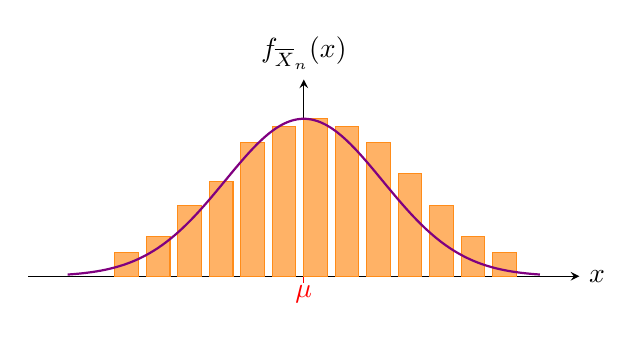
\begin{tikzpicture}[>=stealth, scale=1]
\begin{scope}[yshift=-4.5cm]

% Assi
\draw[->] (-3.5,0) -- (3.5,0) node[right] {$x$};
\draw[->] (0,0) -- (0,2.5) node[above] {$f_{\overline{X}_n}(x)$};

% Punto mu sull'asse x
\draw[red] (0,-0.08) -- (0,0.08);
\node[below, red] at (0,0) {$\mu$};

% Istogramma "a mano" (barre arancioni)
\foreach \x/\h in {-2.4/0.3, -2.0/0.5, -1.6/0.9, -1.2/1.2, -0.8/1.7,
                   -0.4/1.9,  0.0/2.0,  0.4/1.9,  0.8/1.7,  1.2/1.3,
                    1.6/0.9,  2.0/0.5,  2.4/0.3} {
  \draw[fill=orange!60, draw=orange!90]
    (\x,0) rectangle (\x+0.3,\h);
}

% Curva gaussiana approssimata (linea viola)
\draw[domain=-3:3, smooth, samples=100, thick, violet]
  plot (\x,{2.0*exp(-0.5*\x*\x)});
\end{scope}

\end{tikzpicture}
\end{figure}

\bigskip
\noindent \(\bigstar \;\) Il caso degenere in cui $\sigma^2 = 0$ non può essere trattato usando il TCL, in quanto cadono le ipotesi. È però un caso di facile trattazione, infatti avere varianza nulla implica che $X_n \equiv \mu$, e di conseguenza $\overline{X}_n\equiv \mu$.

\bigskip
\noindent \(\bigstar \;\) Il TCL è chiaramente valido anche nel caso in cui non si abbia la media campionaria normalizzata: basta semplicemente fare la normalizzazione:
\[\mathbb P(\overline{X}_n\leq x) = \mathbb P\left(\frac{\overline{X}_n  - \mu}{\sqrt{\frac{\sigma^2}n}}\leq \frac{x  - \mu}{\sqrt{\frac{\sigma^2}n{}}}\right)\approx \Phi\left(\frac{x  - \mu}{\sqrt{\frac{\sigma^2}n{}}}\right)\]
Indirettamente conosciamo pure la legge della media campionaria!

\bigskip
\noindent \(\bigstar \;\) Ragionando in maniera molto simile all'osservazione precedente, possiamo conoscere anche la legge della somma parziale $S_n := (X_1+\cdots+X_n) = n \overline{X}_n$. Basta effettuare una normalizzazione del tipo:
\[\frac{S_n  - n\mu}{\sqrt{n\sigma^2}} = \frac{n(\overline{X}_n -\mu)}{n\sqrt{\frac{\sigma^2}{n}}} = \frac{\overline{X}_n  - \mu}{\sqrt{\frac{\sigma^2}n}} = T_n\]
\[\Rightarrow \qquad \mathbb{P}(S_n\leq x) = \mathbb{P}\left(\frac{S_n  - n\mu}{\sqrt{n\sigma^2}}\leq \frac{x  - n\mu}{\sqrt{n\sigma^2}}\right)\overset{\text{TCL}}{\approx} \Phi\left(\frac{x - n\mu}{\sqrt{n\sigma^2}}\right)\] 

\bigskip
\noindent $\bigstar$\; Dato un qualsiasi campione di variabili aleatorie $X_n\in L^2$, abbiamo visto che, per la LFGN, $\overline{X}_n \;\overset{\mathrm{qc}}{\longrightarrow}\; \mu,$ e che la varianza della media campionaria tende a zero. Di conseguenza, la distribuzione di $\overline{X}_n$ si concentra sempre più attorno a $\mu$ e converge alla misura di Dirac $\delta_\mu$.

\medskip
\noindent Normalizzando, impediamo (grazie al Teorema del Limite Centrale) che la distribuzione collassi in una Dirac:
\[
\frac{\overline{X}_n - \mu}{\sqrt{\sigma^{2}/n}}
\;\overset{\mathcal{L}}{\longrightarrow}\; Z \neq 0.
\]

\medskip
\noindent In un certo senso, è come se stessimo ``intercettando'' la velocità di convergenza in legge. Infatti, dalla LFGN si ha $\overline{X}_n - \mu \;\overset{\mathrm{qc}}{\longrightarrow}\; 0,$ ma poiché la normalizzazione \(\sqrt{n}\,(\overline{X}_n - \mu)\) non converge a una Dirac, e anzi ammette un limite non degenere, ciò implica che lo scostamento $\overline{X}_n - \mu$ converge a zero con ordine
\[
\overline{X}_n - \mu = O_p\!\left(\frac{1}{\sqrt{n}}\right).
\]

In altre parole, il fattore $\sqrt{n}$ rivela esattamente la velocità con cui la media campionaria si avvicina alla sua media.

